%{Software Architecture }

The high–level functionality and control of the robot are implemented in ROS packages. The Robot Operating System (ROS) is a standard and open–source operating system for robot control \cite{9}. ROS is not an operating system in the traditional sense of process management and scheduling; rather, it provides a structured communication layer above the host operating systems of a heterogeneous compute cluster. Our software ROS packages interact with each of the subsystems in C++ and Python for direct system control. The system described uses a Linux based software framework as an operating system (OS) for providing the advantages of using an OS, which supports developing additional modules that can be easily implemented and integrated. 

\section{Robot Operating System (ROS)}

Robot Operating System (ROS) provides operating system like service for the robot. It is a meta-operating system, which loads on top of an operating system, including hardware abstraction, low-level device control, implementation of commonly-used functionality, message-passing between processes, and package management. It also provides tools and libraries for obtaining, building, writing, and running code across multiple computers. These facilities cannot only help robots but also other embedded systems with a rich set of tools to successfully manage the complexity. With ROS handling the basic communications and data exchange.

ROS currently only runs on Unix-based platforms. Software for ROS is primarily tested on Ubuntu and Mac OS X systems, though the ROS community has been contributing support for Fedora, Gentoo, Arch Linux and other Linux platforms. While a port to Microsoft Windows for ROS is possible, it has not yet been fully explored.

The core ROS system, along with useful tools and libraries are regularly released as a ROS Distribution. This distribution is similar to a Linux distribution and provides a set of compatible software for others to use and build upon example for this distribution: Hydro, Indigo, Jade, Kinetic, Lunar...etc. [http://wiki.ros.org]

Our choice was Kinetic because is the update  distribution that have a LTS with high variety of support from ROS community that make it easy to exchange the knowledge and figure out how to solve issues and to come up with new idea to implement it. 
\subsection{Why ROS?}
	The answer for this question lies in power of ROS the make it preferable for most of the designers: 
  
	\begin{description}
		\item [Inter-platform operability]: ROS message-passing means that you can work between very different components and subsystems that are probably running with different languages (maybe something like low-level hardware control with C for speed, and high-level state machines with Java or Python for ease of coding). This also gets around the problem of the mess of APIs you would have had to deal with before.
		
		\item [Modularity]: Since things are connected by a distributed message system, if one component crashes, your whole system doesn't crash. Granted, there are plenty of ways to make your system more robust so that this doesn't happen in the first place, but ROS makes it easier for your robot to continue doing its thing even if two sensors and an arm motor have died (for example).
		
		\item [Concurrent resource handling]: Without ROS, reading/writing to resources quickly becomes a mess with large multi-threaded systems (i.e. virtually any robotics application). Again, there are ways to deal with this, but ROS simplifies the whole process by ensuring that your threads aren't actually trying to read and write to shared resources, but are rather just publishing and subscribing to messages.
		\item[ Vibrant Community]: Over the past several years, ROS has grown to include a large community of users worldwide. Historically, the majority of the users were in research labs, but increasingly we are seeing adoption in the commercial sector, particularly in industrial and service robotics.
		
		\item [Collaborative Environment]: ROS by itself offers a lot of value to most robotics projects, but it also presents an opportunity to network and collaborate with the world class roboticists that are part of the ROS community. One of the core philosophies in ROS is shared development of common components.
	\end{description}
Interested reader can find more information,material, and much more at:  \url{www.ros.org/core-components}

\subsection{ROS Package}
	Software in ROS is organized in packages. A package might contain ROS nodes, a ROS-independent library, a dataset, configuration files, a third-party piece of software, or anything else that logically constitutes a useful module. The goal of these packages it to provide this useful functionality in an easy-to-consume manner so that software can be easily reused. In general, ROS packages follow a "Goldilocks" principle: enough functionality to be useful, but not too much that the package is heavyweight and difficult to use from other software.
	
	Packages are easy to create by hand or with tools like catkin\_create\_pkg. A ROS package is simply a directory descended from ROS\_PACKAGE\_PATH (see ROS Environment Variables) that has a package.xml file in it. Packages are the most atomic unit of build and the unit of release. This means that a package is the smallest individual thing you can build in ROS and it is the way software is bundled for release (meaning, for example, there is one debian package for each ROS package), respectively.
	
\subsection{ROS Node}
	
	A node is a process that performs computation. Nodes are combined together into a graph and communicate with one another using streaming topics, RPC services, and the Parameter Server. These nodes are meant to operate at a fine-grained scale; a robot control system will usually comprise many nodes. For example, one node controls a laser range-finder, one Node controls the robot's wheel motors, one node performs localization, one node performs path planning, one node provide a graphical view of the system, and so on.
	
	The use of nodes in ROS provides several benefits to the overall system. There is additional fault tolerance as crashes are isolated to individual nodes. Code complexity is reduced in comparison to monolithic systems. Implementation details are also well hidden as the nodes expose a minimal API to the rest of the graph and alternate implementations, even in other programming languages, can easily be substituted.
	
	All running nodes have a graph resource name that uniquely identifies them to the rest of the system. For example, /hokuyo\_node could be the name of a Hokuyo driver broadcasting laser scans. Nodes also have a node type, that simplifies the process of referring to a node executable on the fileystem. These node types are package resource names with the name of the node's package and the name of the node executable file. In order to resolve a node type, ROS searches for all executables in the package with the specified name and chooses the first that it finds. As such, you need to be careful and not produce different executables with the same name in the same package. Finally, a ROS node is written with the use of a ROS client library, such as roscpp or rospy.
	
\subsection{Publisher/Subscriber}
	The Publisher object represents a publisher on the ROS network. The object publishes to an available topic or to a topic that it creates. This topic has an associated message type. When the Publisher object publishes a message to the topic, all subscribers to the topic receive this message. The same topic can have multiple publishers and subscribers.
	
	The primary mechanism for ROS nodes to exchange data is to send and receive messages. Messages are transmitted on a topic and each topic has a unique name in the ROS network. If a node wants to share information, it will use a publisher to send data to a topic. A node that wants to receive that information will use a subscriber to that same topic. Besides its unique name, each topic also has a message type, which determines the types of messages that are allowed to be transmitted.
	
	This publisher/subscriber communication has the following characteristics:
	\begin{enumerate}
		\item Topics are used for many-to-many communication. Many publishers can send messages to the same topic and many subscribers can receive them.
		\item Publisher and subscribers are decoupled through topics and can be created and destroyed in any order. A message can be published to a topic even if there are no active subscribers.
	\end{enumerate}
	
	The concept of topics, publishers, and subscribers is illustrated in the figure.\ref{Pub}.
	\begin{figure}[h]		
		\centering
		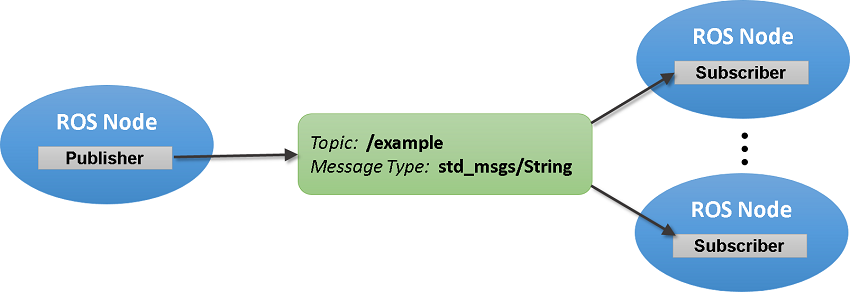
\includegraphics[width =.8\textwidth]{publish_subscribe_concept}
		\caption{publish subscribe concept}
		\label{Fig:Pub}
	\end{figure}


\subsection{ROS Topic}

	Topics are named buses over which nodes exchange messages. Topics have anonymous publish/subscribe semantics, which decouples the production of information from its consumption. In general, nodes are not aware of who they are communicating with. Instead, nodes that are interested in data subscribe to the relevant topic; nodes that generate data publish to the relevant topic. There can be multiple publishers and subscribers to a topic.
	
	Topics are intended for unidirectional, streaming communication. Nodes that need to perform remote procedure calls, i.e. receive a response to a request, should use services instead. There is also the Parameter Server for maintaining small amounts of state.
	
	Each topic is strongly typed by the ROS message type used to publish to it and nodes can only receive messages with a matching type. The Master does not enforce type consistency among the publishers, but subscribers will not establish message transport unless the types match. Furthermore, all ROS clients check to make sure that an MD5 computed from the msg files match. This check ensures that the ROS Nodes were compiled from consistent code bases.
	
	with a simple words we can define this terms:\\
	
	Nodes: A node is an executable that uses ROS to communicate with other nodes.
	Topics: Nodes can publish messages to a topic as well as subscribe to a topic to receive messages.
	Messages: ROS data type used when subscribing or publishing to a topic.
	Master: The ROS Master provides name registration and lookup to the rest of the Computation Graph. Without the Master, nodes would not be able to find each other, exchange messages, or invoke services.
	roscore: is a collection of nodes and programs that are pre-requisites of a ROS-based system. You must have a roscore running in order for ROS nodes to communicate. It is launched using the roscore command.
	
	

\subsection{Can we access ROS form a remote computer?}
	ROS is a distributed computing environment. A running ROS system can comprise dozens, even hundreds of nodes, spread across multiple machines. Depending on how the system is configured, any node may need to communicate with any other node, at any time.	
	\begin{itemize}
		\item There must be complete, bi-directional connectivity between all pairs of machines, on all ports.
		\item Each machine must advertise itself by a name that all other machines can resolve.
	\end{itemize}

More information can be found at:  \url{wiki.ros.org/ROS/NetworkSetup}

\section{UNIX}
	UNIX is an open source operating system which was first developed in the 1960s, and has been under constant development ever since. By operating system, we mean the suite of programs which make the computer work. It is a stable, multi-user, multi-tasking system for servers, desktops and laptops.
	UNIX systems also have a graphical user interface (GUI) similar to Microsoft Windows which provides an easy to use environment. However, knowledge of UNIX is required for operations which aren't covered by a graphical program, or for when there is no windows interface available.
	
	- Types of UNIX
	
	There are many different versions of UNIX, although they share common similarities. The most popular varieties of UNIX are Sun Solaris, GNU/Linux, Ubuntu, Kali, and MacOS X.
	Here in the School, we use Solaris on our servers and workstations, and Fedora Linux on the servers and desktop PCs.
	
	- The UNIX operating system
	The UNIX operating system is made up of three parts; the kernel, the shell and the programs.
	
	- The kernel
	The kernel of UNIX is the hub of the operating system: it allocates time and memory to programs and handles the filestore and communications in response to system calls.
	
	- The shell
	The shell acts as an interface between the user and the kernel. The shell is a command line interpreter (CLI), it interprets the commands the user types in and arranges for them to be carried out.
	

\section{General View Of The Control System}

The control system of the robot can be divided into two parts:

\begin{itemize}
\item Raspberry Pi - High level -
\item Arduino - Low level -
\end{itemize}

All computing and control operation is done on RPi and Arduino that lies on the robot to inure the speed of control and precision.
The sensors data send from mobile App to the RPi through TCP/IP connection and to a computer also, RPi receive this data and process it to be aware with its environment and make a decision upon it, the computer show this data on a GUI to the operator/user so he can also make a decision using the reading form sensors and the camera.
When a order form an operator using Joystick/Bluetooth to move the robot the RPi take this order and send it to the Arduino through a serial port, using a C++ program in Arduino we compute the angles to move to the desired direction with minimal error. Figure\ref{Fig:Outline} show an Outline for the control system.

\begin{figure}[h]		
	\centering
	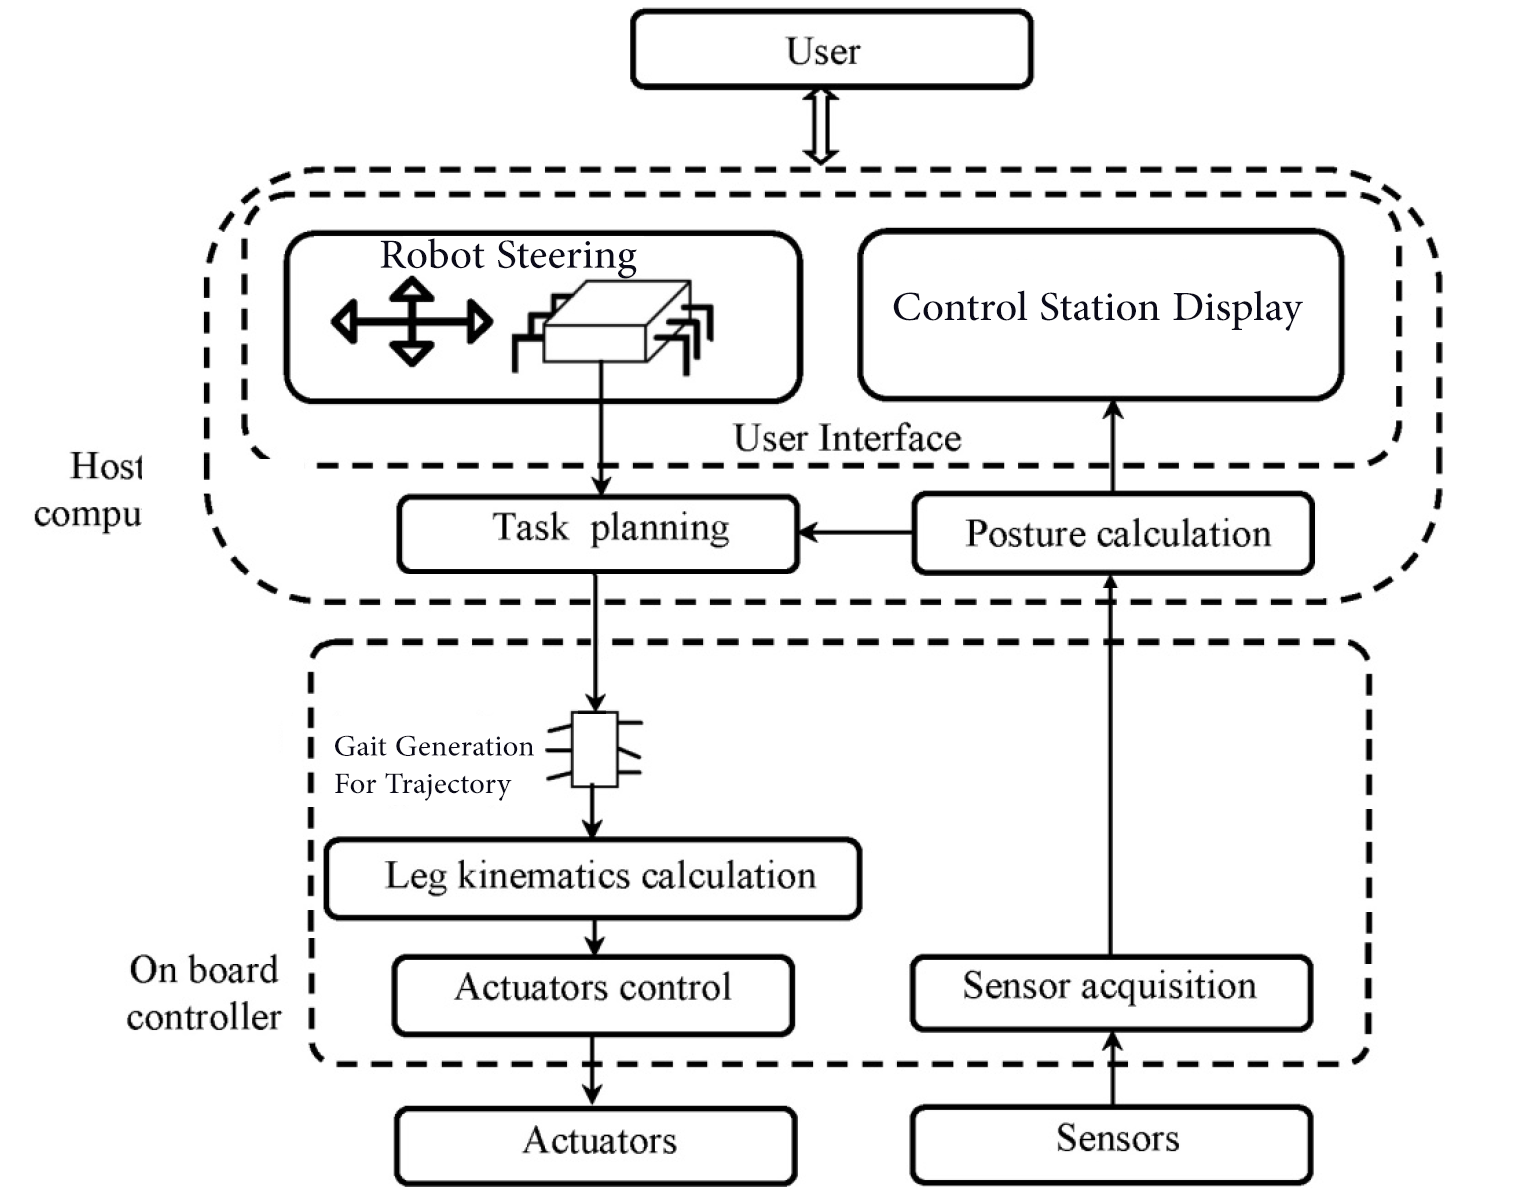
\includegraphics[width =.8\textwidth]{OCS}
	\caption{Outline of control systems.}
	\label{Fig:Outline}
\end{figure}


\subsection{Raspberry Pi}

A Raspberry Pi is a credit card-sized computer originally designed for education, inspired by the 1981 BBC Micro. Creator Eben Upton's goal was to create a low-cost device that would improve programming skills and hardware understanding. But thanks to its small size and accessible price, it was quickly adopted by tinkerers, makers, and electronics enthusiasts for projects that require more than a basic microcontroller.

The Raspberry Pi is slower than a modern laptop or desktop but is still a complete Linux computer and can provide all the expected abilities that implies, at a low-power consumption level.

The Raspberry Pi is open hardware, with the exception of the primary chip on the Raspberry Pi, the Broadcomm SoC (System on a Chip), which runs many of the main components of the board–CPU, graphics, memory, the USB controller, etc. Many of the projects made with a Raspberry Pi are open and well-documented as well and are things you can build and modify yourself.

\begin{itemize}
	\item What kind of operating system does the Raspberry Pi run?\\
	
	The Raspberry Pi was designed for the Linux operating system, and many Linux distributions now have a version optimized for the Raspberry Pi.
	
	Two of the most popular options are Raspbian, which is based on the Debian operating system, and Pidora, which is based on the Fedora operating system. For beginners, either of these two work well; which one you choose to use is a matter of personal preference. A good practice might be to go with the one which most closely resembles an operating system you’re familiar with, in either a desktop or server environment.
	
	If you would like to experiment with multiple Linux distributions and aren't sure which one you want, or you just want an easier experience in case something goes wrong, try NOOBS, which stands for New Out Of Box Software. When you first boot from the SD card, you will be given a menu with multiple distributions (including Raspbian and Pidora) to choose from. If you decide to try a different one, or if something goes wrong with your system, you simply hold the Shift key at boot to return to this menu and start over.
	
	There are, of course, lots of other choices. OpenELEC and RaspBMC are both operating system distributions based on Linux that are targeted towards using the Raspberry Pi as a media center. There are also non-Linux systems, like RISC OS, which run on the Pi. Some enthusiasts have even used the Raspberry Pi to learn about operating systems by designing their own.
\end{itemize}

% Take this to the Component Part 
	Raspberry Pi 3 Model B specification
	The Raspberry Pi 3 Model B is the third generation Raspberry Pi. This powerful credit-card sized single board computer can be used for many applications and supersedes the original Raspberry Pi Model B+ and Raspberry Pi 2 Model B. Whilst maintaining the popular board format the Raspberry Pi 3 Model	B brings you a more powerful processer, 10x faster than the first generation Raspberry Pi. Additionally it adds wireless LAN \& Bluetooth connectivity making it the ideal solution for powerful connected designs.
\begin{figure}[h]
\centering
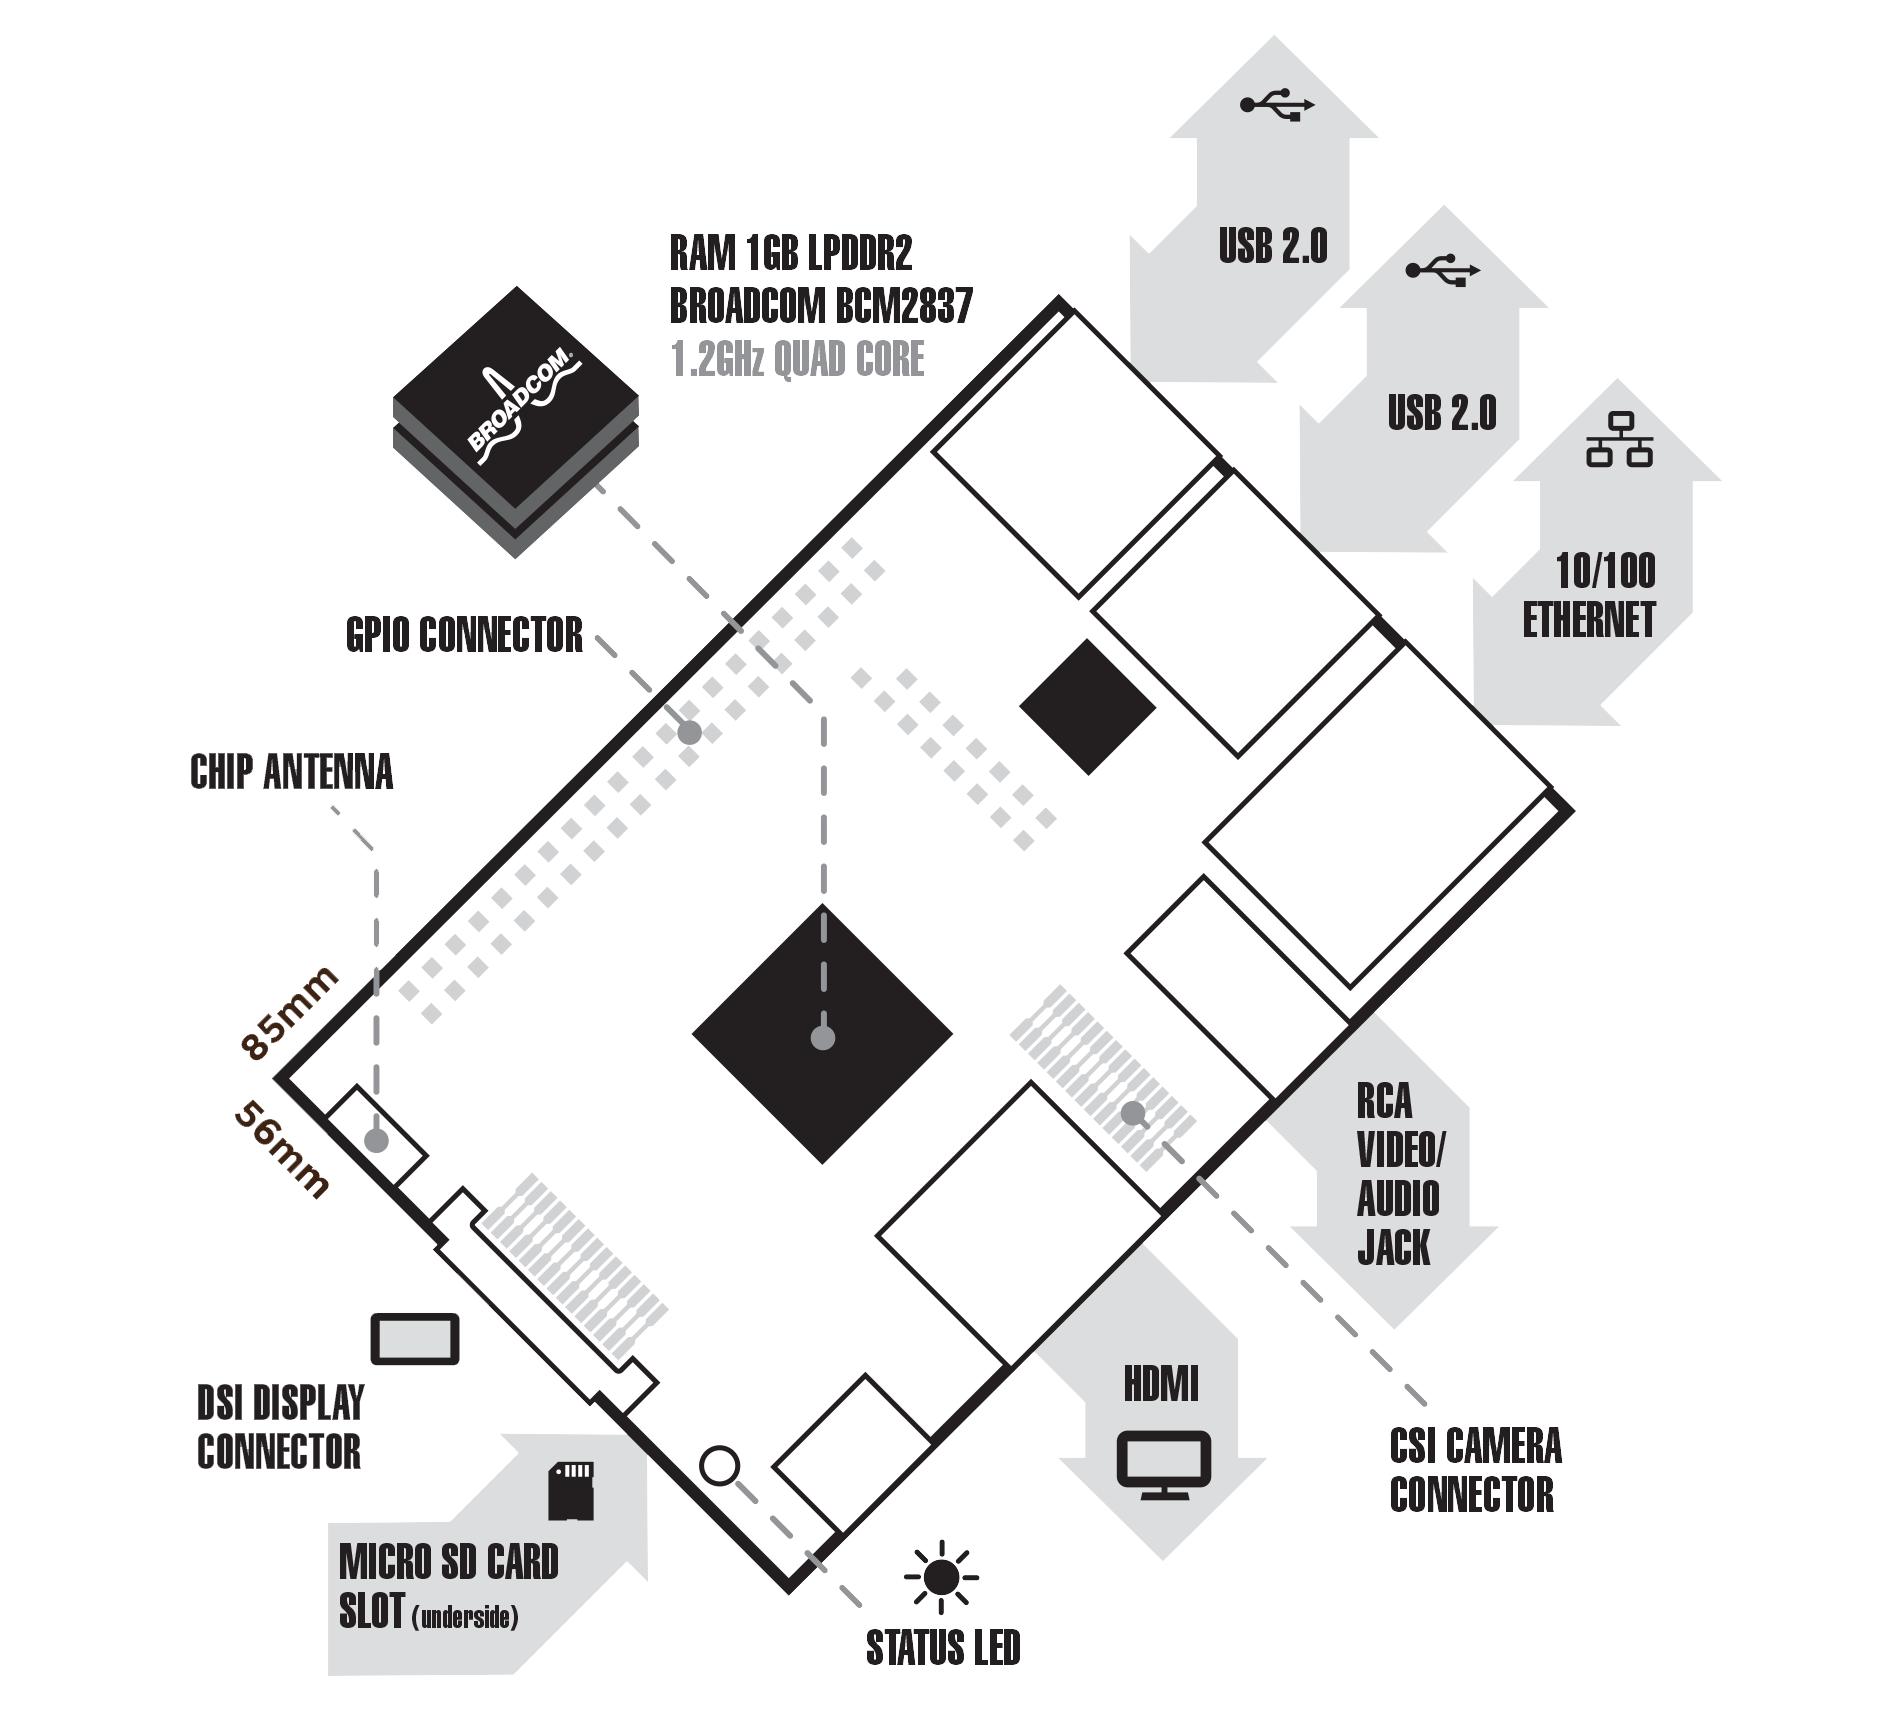
\includegraphics[width =.8\textwidth]{RP3}
\caption{Raspberry Pi 3 Model B.}
\label{Fig:RP3}
\end{figure}
\begin{center}
\begin{tabular}{ |l||p{12cm}|}
	\hline
	Processor      & Broadcom BCM2387 chipset. 1.2GHz Quad-Core ARM Cortex-A53 802.11 b/g/n Wireless LAN and Bluetooth 4.1 (Bluetooth Classic and LE)\\ \hline
	GPU               & Dual Core VideoCore IV® Multimedia Co-Processor. Provides Open GL ES 2.0, hardware-accelerated OpenVG, and 1080p30 H.264 high-profile decode. \\ \hline
	Memory          & 1GB LPDDR2  \\ \hline
	Operating System  & Boots from Micro SD card, running a version of the Linux operating system  \\ \hline
	Dimensions     & 85 x 56 x 17mm  \\ \hline
	Power             & Micro USB socket 5V1, 2.5A  \\ \hline
	Ethernet          & 10/100 BaseT Ethernet socket  \\ \hline
	Video Output   & HDMI (rev 1.3 \& 1.4 Composite RCA (PAL and NTSC)  \\ \hline
	Audio Output   & Audio Output 3.5mm jack, HDMI     \\ \hline
	USB                 & 4 x USB 2.0 Connector   \\ \hline
	GPIO Connector    & 40-pin 2.54 mm (100 mil) expansion header: 2x20 strip Providing 27 GPIO pins as well as +3.3 V, +5 V and GND supply lines \\ \hline
	Camera Connector  & 15-pin MIPI Camera Serial Interface (CSI-2) \\ \hline
	Display Connector & Display Serial Interface (DSI) 15 way flat flex cable connector with two data lanes and a clock lane    \\ \hline
	Memory Card       & Slot Push/pull Micro SDIO  \\ \hline
\end{tabular}
\end{center}

	\subsubsection{Ubuntu MATE with Raspberry Pi}
	Ubuntu MATE is a stable, easy-to-use operating system with a configurable desktop environment. It is ideal for those who want the most out of their computers and prefer a traditional desktop metaphor. With modest hardware requirements it is suitable for modern workstations, single board computers and older hardware alike. Ubuntu MATE makes modern computers fast and old computers usable.
	
	The MATE desktop is essentially a continuation of the traditional Gnome 2 desktop environment. Combining the MATE desktop with Ubuntu gives you an experience that is almost identical to the early days of Ubuntu, prior to the switch to Unity.
	
	Martin Wimpress and Rohith Madhavan have made an Ubuntu MATE image for the Raspberry Pi 2 and Raspberry Pi 3 based on the regular Ubuntu armhf base, not the new Ubuntu “Snappy” Core, which means that the installation procedure for applications uses the traditional tools, ie apt-get with highly recommended microSDHC Class 6 or Class 10 microSDHC card. Ubuntu MATE 16.04 also fully supports the built-in Bluetooth and Wifi on the Raspberry Pi 3 and features hardware accelerated video playback in VLC and hardware accelerated decoding and encoding in ffmpeg
	
	To installing Ubuntu MATE onto Raspberry Pi 3, starting by download the OS into microSD then the partition is automatically resized to fill your microSD card when the pi is powered up for the first time, typical guided installer is shown up. Installation takes several minutes and finally the system reboots and you arrive at the desktop. A Welcome app provides some good information on Ubuntu MATE, including a section specific for the Raspberry Pi.
	
	The Welcome app explains that the while the system is based on Ubuntu MATE and uses Ubuntu armhf base, it is in fact using the same kernel as Raspian. It also turns out that a whole set of Raspian software has been ported over such as raspi-config, rpi.gpio, sonic-pi, python-sent-hat, omxplayer, etc.
	
	[ubuntu-mate.org/blog/ubuntu-mate-xenial-raspberry-pi]
	
	\subsubsection{Raspberry Pi with ROS} 
	
	This part is consider as the the brain of the robot as it contain all the nodes of our robot that make it move and interact with its environment, we can divide our program to two main packages that will control all functions in our robot:
	
	\begin{enumerate}
		\item Movement package \\ 
			This package is responsible to handle the movement of the robot, as it takes the input form joystick/bluetooth and using node Joystick it publish the wanted button to the low level Hardware to do an action upon the received button.
			
			this package have tow nodes, the first one on the RPi which handle the joystick/bluetooth part of taking command, the second node is on Arduino which receive the command and handle the action of movement as wanted.
			
			An Extra topic is add to the Arduino node to handle the ultrasonic sensor reading for more known of the environments variables. 
			\begin{figure}[h]		
				\centering
				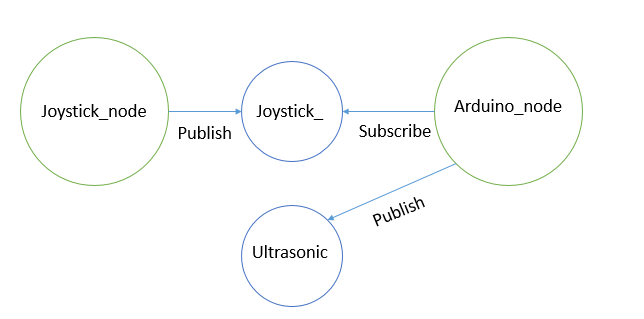
\includegraphics[width =.8\textwidth]{Movement_pck}
				\caption{General view of Movement Package.}
				\label{Fig:Movement}
			\end{figure}
		\item Client package  \\
			This package is responsible to handle the communication through the TCP/IP connection, this package is consist of two way of communication, so it receive the sensor data as will be descried in the Mobile Application section then it publish these data to the GUI node which can also select some sensor id or all sensors to be receive then publish it value to the Client node to git its value(s) form the mobile application.
			\begin{figure}[h]		
				\centering
				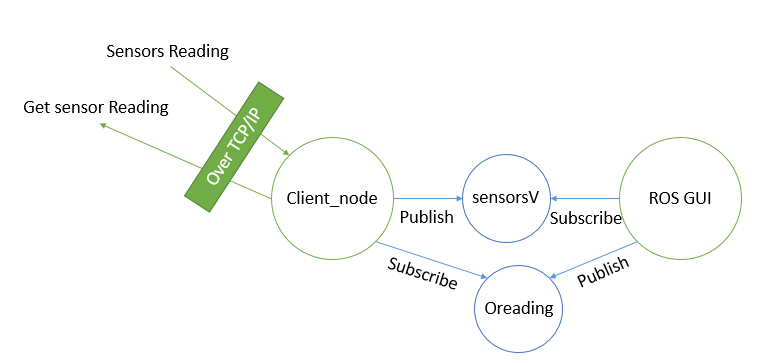
\includegraphics[width =.8\textwidth]{Client_pck}
				\caption{General view of Client Package.}
				\label{Fig:Client}
			\end{figure}  
	\end{enumerate}

\subsection{Arduino Mega}
Arduino is an open-source platform used for building electronics projects. Arduino consists of both a physical programmable circuit board (often referred to as a microcontroller) and a piece of software, or IDE (Integrated Development Environment) that runs on your computer, used to write and upload computer code to the physical board.

The Arduino platform has become quite popular with people just starting out with electronics, and for good reason. Unlike most previous programmable circuit boards, the Arduino does not need a separate piece of hardware (called a programmer) in order to load new code onto the board – you can simply use a USB cable. Additionally, the Arduino IDE uses a simplified version of C++, making it easier to program. 
Finally, Arduino provides a standard form factor that breaks out the functions of the micro-controller into a more accessible package.

The Arduino Mega 2560 is a microcontroller board based on the ATmega2560. It has 54 of digital input/output pins (14 can be used as PWM outputs), 16 analog inputs, a USB connection, a power jack,a 16 MHz crystal oscillator, and a reset button. It contains everything needed to support the microcontroller; simply connect it to a computer with a USB cable or power it with a AC-to-DC adapter or battery to get started. The large number of pins make this board very handy for projects that require a bunch of digital inputs or outputs.


\begin{figure}[h]		
	\centering
	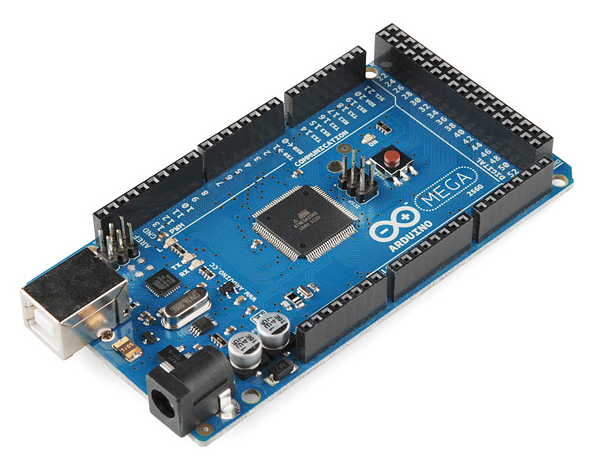
\includegraphics[width =.8\textwidth]{Arduino_Mega}
	\caption{Arduino Mega.}
	\label{Fig:Mega}
\end{figure}
	 Arduino Mega specification
\begin{center}
	\begin{tabular}{ |c|c|}
		\hline
		Microcontroller			& ATmega2560 \\ \hline
		Operating Voltage		& 5V\\ \hline
		Input Voltage			& (recommended) 7-12V\\ \hline
		Input Voltage (limits) 	& 6-20V\\ \hline
		Digital I/O Pins 		& 54 (of which 14 provide PWM output)\\ \hline
		Analog Input Pins 		& 16\\ \hline
		DC Current per I/O Pin	& 40 mA\\ \hline
		DC Current for 3.3V Pin & 50 mA\\ \hline
		Flash Memory			& 256 KB of which 8 KB used by bootloader\\ \hline
		SRAM					& 8 KB\\ \hline
		EEPROM 					& 4 KB\\ \hline
		Clock Speed 			& 16 MHz\\ \hline
	\end{tabular}
\end{center}

		\subsubsection{Arduino whit Raspberry Pi} 
		
		Rather than struggle with the very basic unprotected IO pins on the Raspberry Pi and the lack of real-time performance in Linux, the ideal setup for many real-world-interfacing projects is Raspberry Pi + Arduino.
		
		There are four basic ways to connect Arduino to Raspberry Pi:
		\begin{enumerate}
			\item Buy an add-on board like the Gertboard which has an Arduino compatible IC on it. Pricey.
			\item Plug a standard Arduino into the USB port of the RPi. This is by far the easiest method and minimises wiring and hassle. However it requires the more expensive Arduinos.
			\item Use a USB to Serial adapter with a cheaper/smaller Arduino like a Pro Mini or a self-made Shrimp. This is the best DIY option and has the same advantage of method 2 that you can power the Arduino/Shrimp from USB.
			\item Use the Serial Pins on the Raspberry Pi to connect to a cheaper/smaller Aruduino like a Pro Mini or a self-made Shrimp. This is theoretically the cheapest method but by far the most hassle. This is also the best method if you are using the cheaper Raspberry Pi Model A and its single USB port is being used for Wifi.
		\end{enumerate}	
		Using the second method to connect the two devices in serial connection,
		
		
		\subsubsection{Arduino PWM to Servo Motors} 
		
		
\section{Mobile Application}

	Most of the android devices have built-in sensors that measure motion, orientation, and various environmental condition.
	SensorsCORE is Android application act like server that read any kind of data from your smartphone's sensors and send it through socket request to any client.  
	
	- How to communicate: 
	
	The communication between SensorsCOER(server) and your application(client) based on socket communication. The server is accessed via server's IP address (or domain name) and a port number. Once two application are connected, they can communicate streams of bytes with each other.  
	
	- How it works: 
	
	Once your application connected with the server for the first time, it send a list of your available sensors in your smartphone - you can use – with its IDs. You can send ID of the desired sensor that you want to get its values to the server. Every time you send a request, you get an answer with the sensor values. So we have three type of requests. 
	The first request sent with first time connection with the list of available sensors and its IDs. 
	When you want a data form specific sensor, you sent a request with the sensor's id The third request is initialized when you want the data from all sensors. 

	Example:
	\begin{figure}[h]		
	\centering
	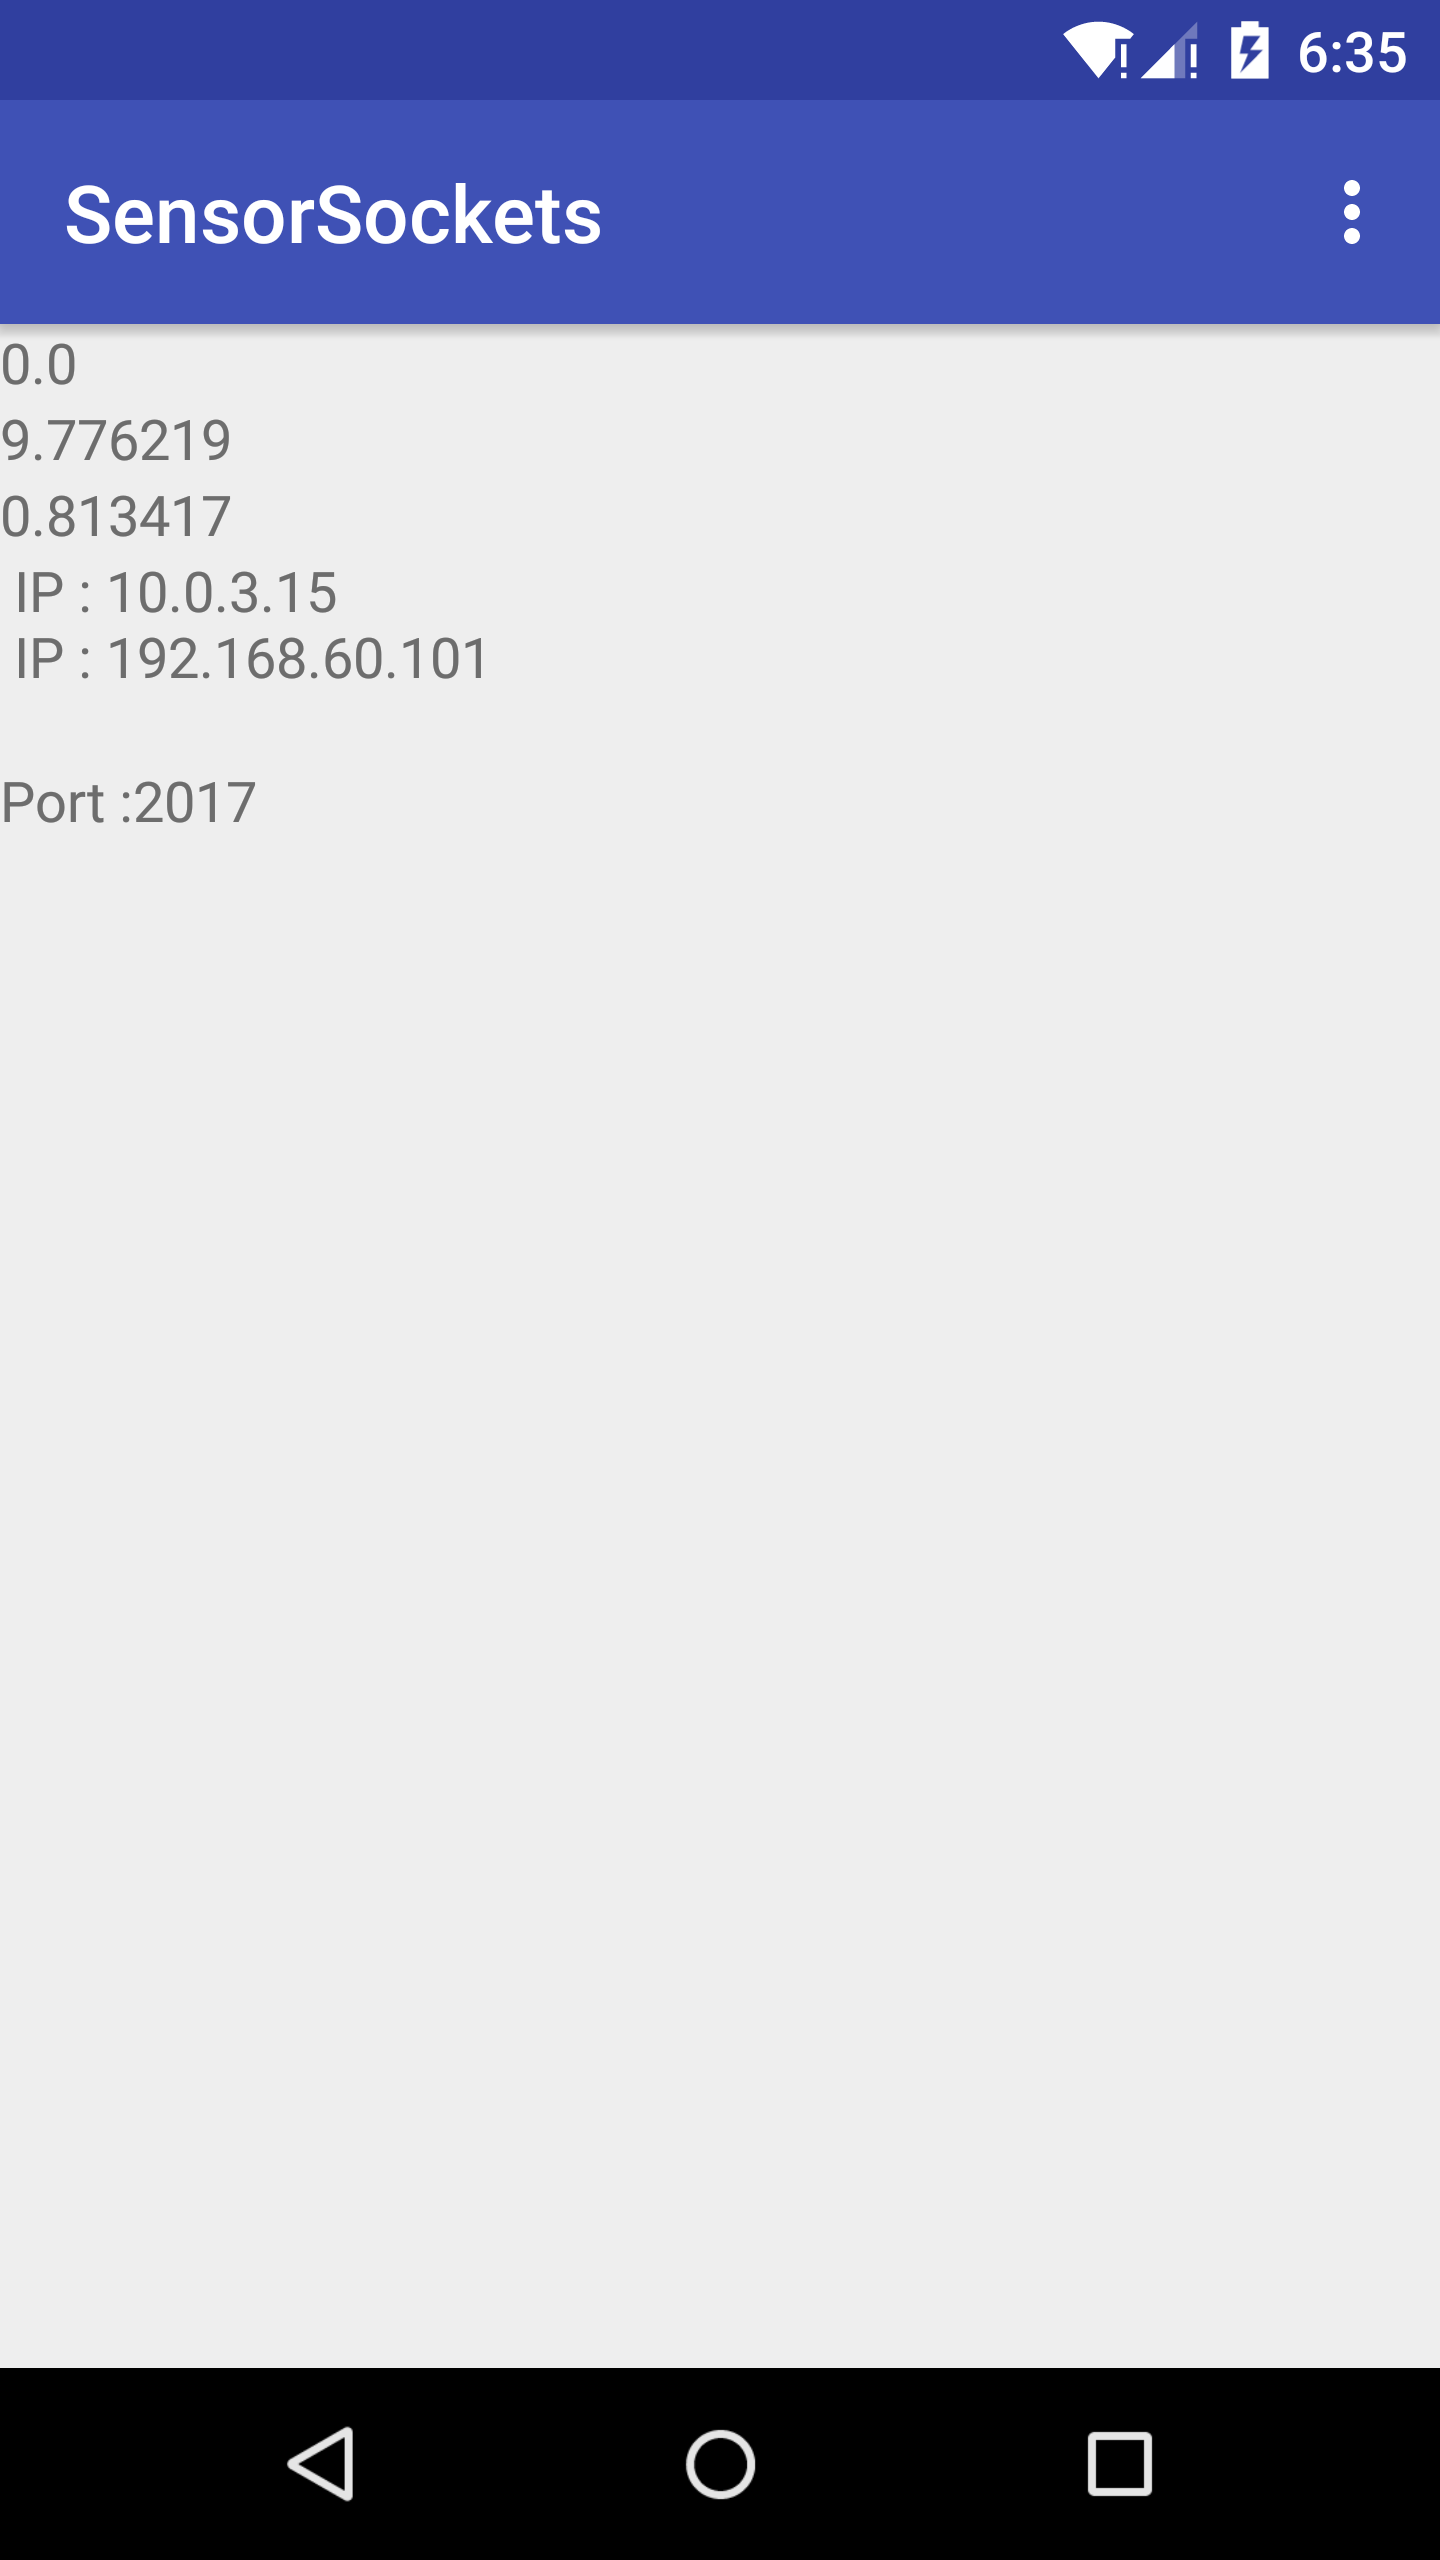
\includegraphics[width =.45\textwidth]{App1}\quad
    	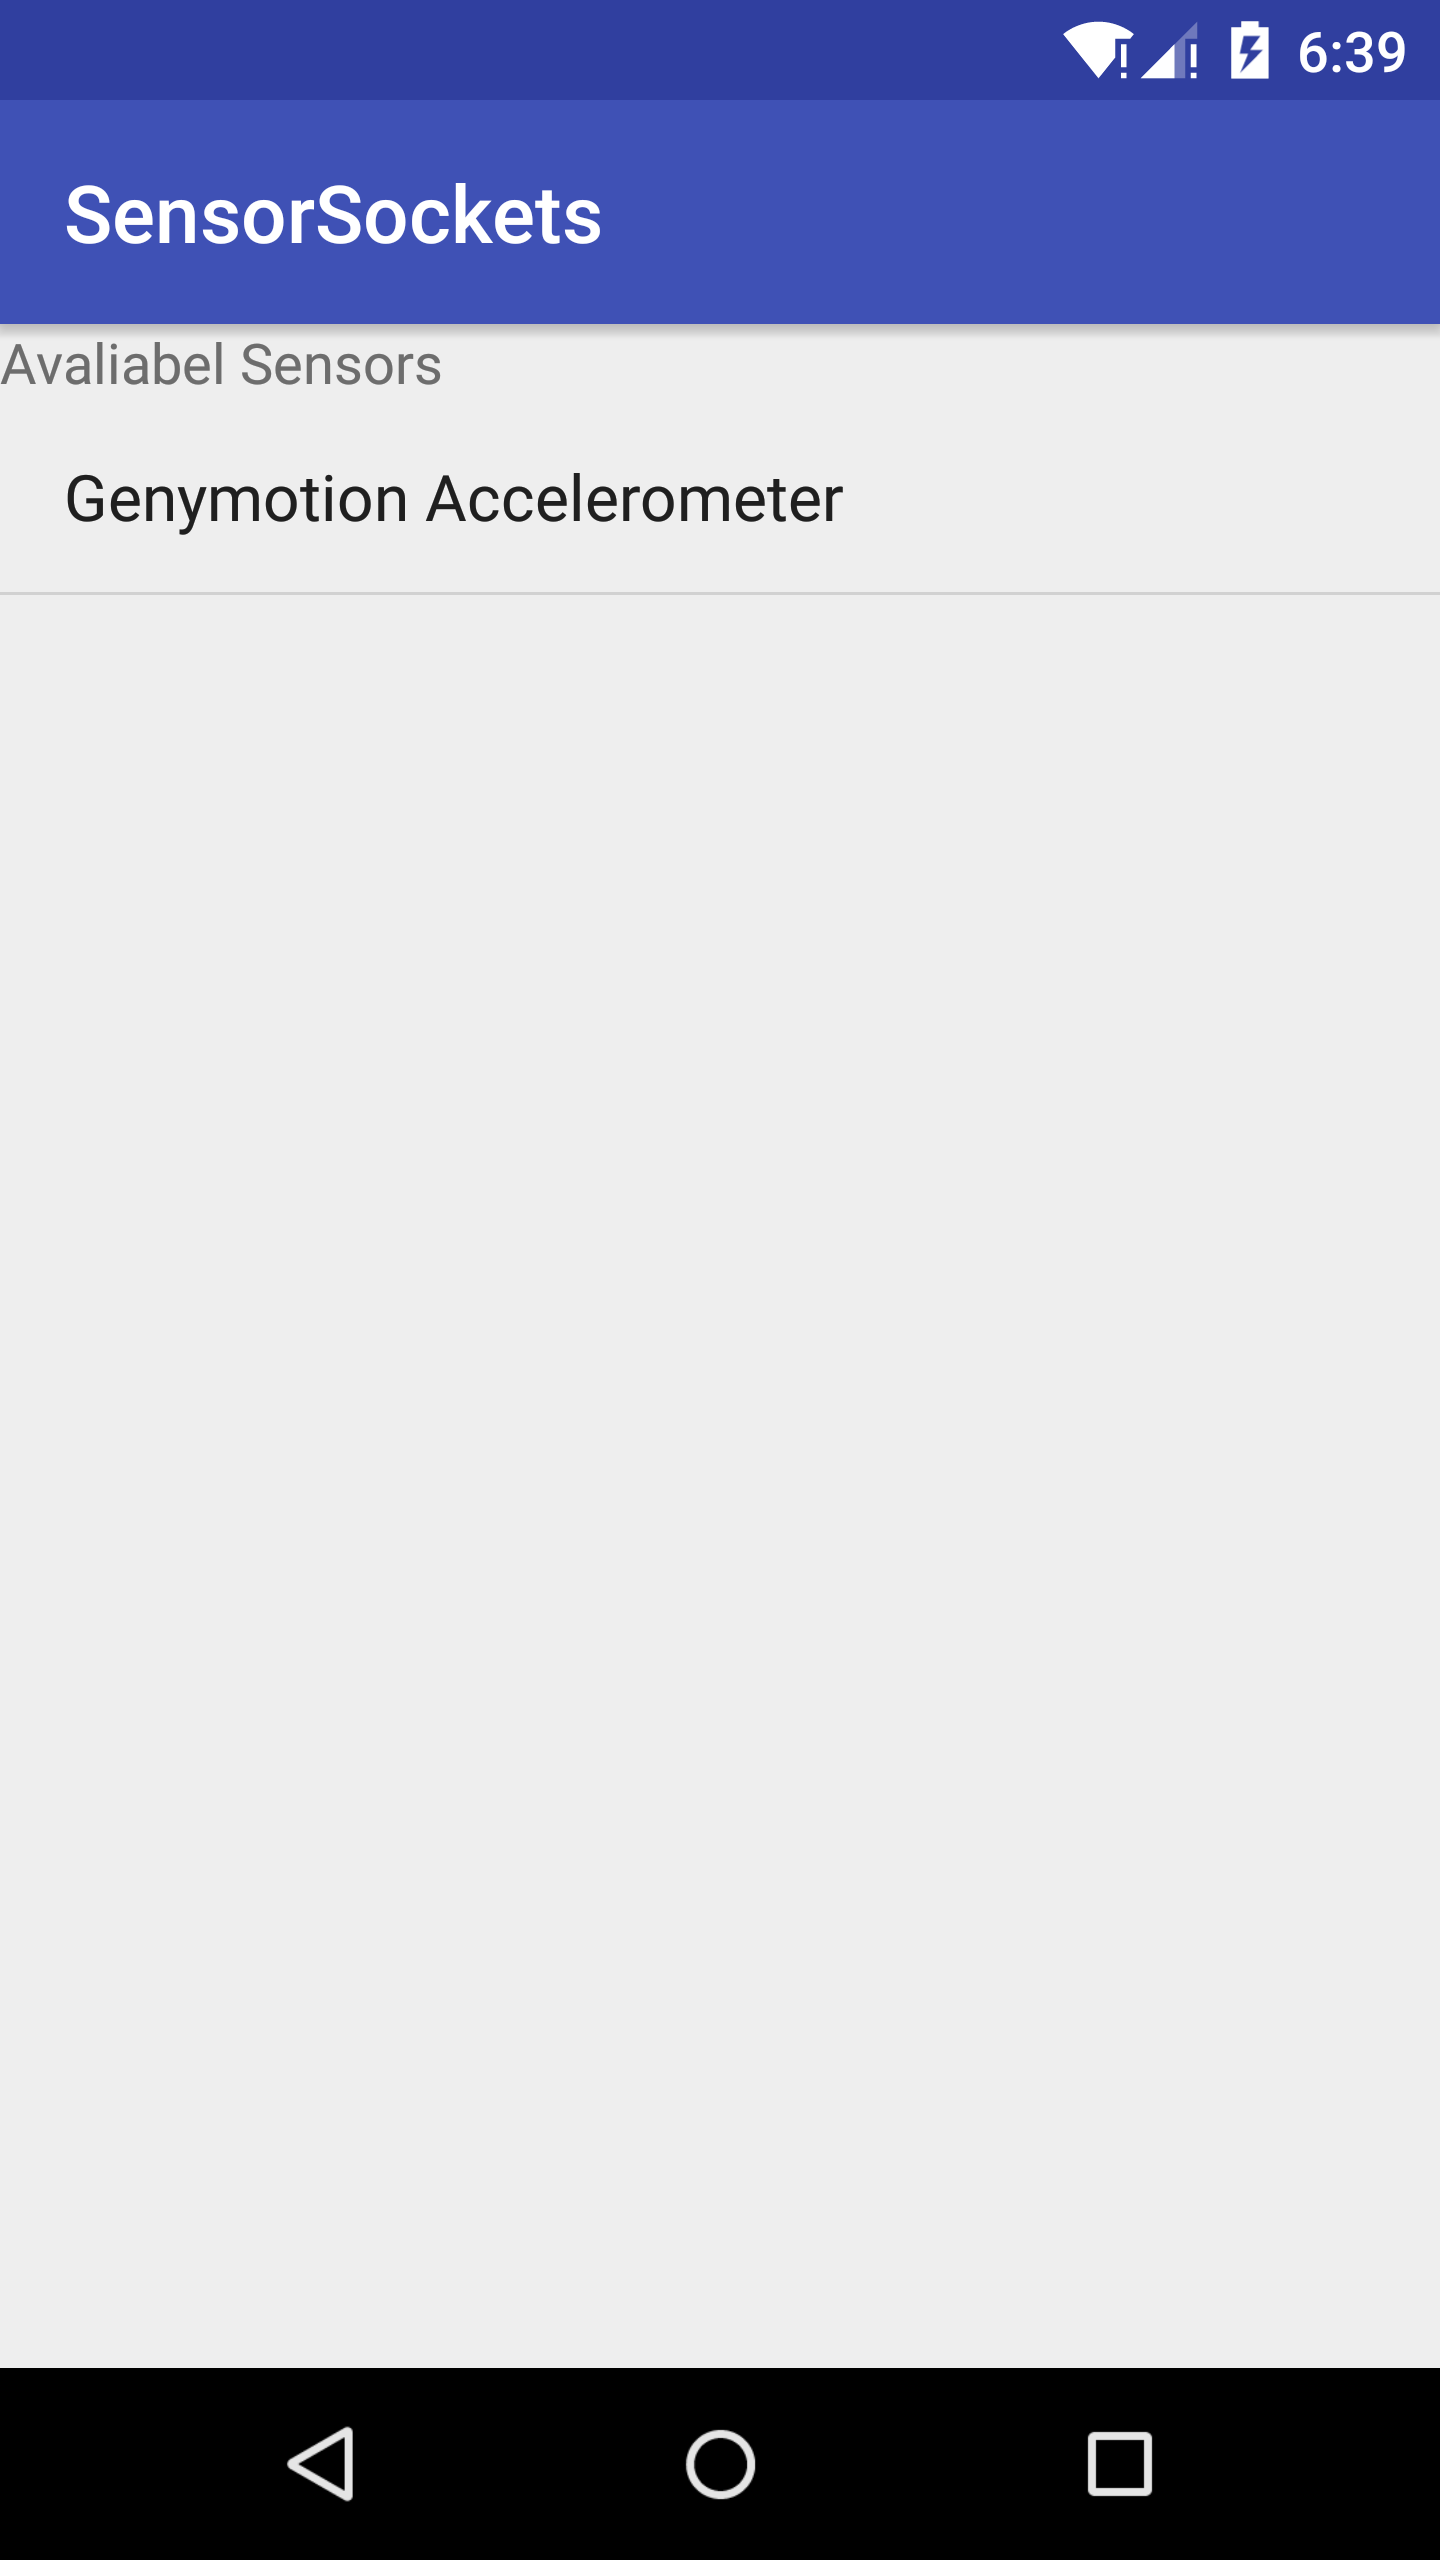
\includegraphics[width =.45\textwidth]{App2}
	\caption{Home page (left) and Sensor window (right)}
	\label{Fig:App1}
\end{figure}




\section{Communication Types}

	
	\subsection{Joystick}
	the wireless joystick communicates with the Raspberry Pi, using a ROS node called ‘joy’, and send a keystroke to it. Then the Raspberry Pi find the key pressed using a python library called ‘pygame’ and send a proper character on the serial port to the Arduino, our low-level interface with the servomotors. Lastly, the Arduino checks the received character and perform the needed action.
	\begin{figure}[h]		
		\centering
		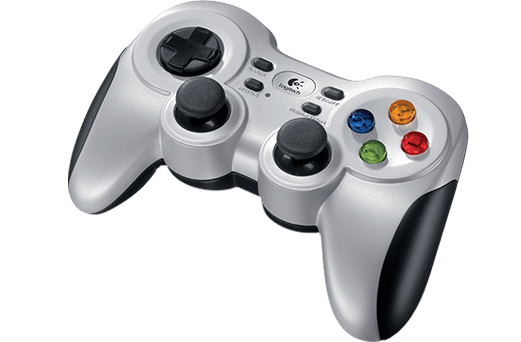
\includegraphics[width =.45\textwidth]{logitech_joy}
		\caption{JoyStick.}
		\label{Fig:joy}
	\end{figure}

	\subsection{BT Joystick}
	Goals:
		Using the Mobile  Bluetooth to control the robot as it contain joystick simulator to send the command to RPi, also this app capable to receive a video recorded form the Mobile on the robot as a background to the joystick so we can control every thing from one app and to see what the robot see.
		
	How it works:
		Using serial communication to Send data between two Bluetooth devices.
		\begin{figure}[h]		
			\centering
			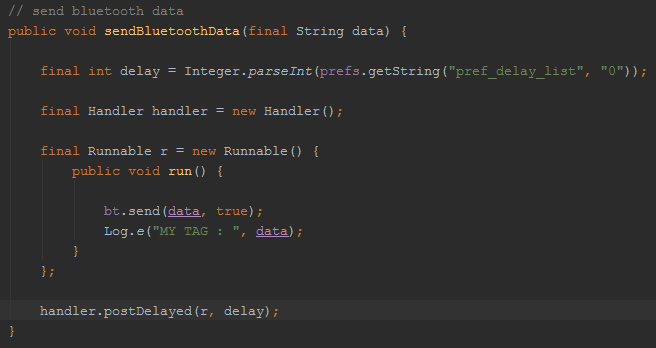
\includegraphics[width =.45\textwidth]{BT_app}
			\caption{Function for sending data through Bluetooth.}
			\label{Fig:BT}
		\end{figure}
		
		First we get the delay value from the setting the user saved.
		We make a handler that schedule the runnable to be executed at some point in the future.
		A new thread is made to send the Bluetooth data called "r" that will use the "bt" model that knows how to deal with Bluetooth then we tell the model to send the data.
		Then the handler will tell the runnable "r" to be executed at some point of the future that time will be determined by the variable "delay".
	How to use the program:
	\begin{itemize}
		\item After opening the program, the program will show you a button to open Bluetooth press "turn on" and confirm opening Bluetooth for your device.
		\item The first thing you need to do is setting and choosing IP and Port that you will connect to.
		\item Remove the port if you will connect to a global server or leave it and choose the right port to connect to in the case of local server.
		\item Now to return to the main activity press run at the bottom-center of the screen and the age is loaded at the background.
		\item Choose a Bluetooth a device to connect to.
		\item Change the joypad buttons look alike config to make ever button send the intended data.
		\item Now use the joypad buttons to control the robot.
	\end{itemize}
		
	\subsection{Wi-Fi}
		Another line of communication is between our control station and an Android smart phone mounted on the robot through a TCP/IP client server application.
		\begin{itemize}
			\item What is TCP/IP?\\
			When two computers follow the same protocols—the same set of rules—they can understand each other and exchange data. TCP/IP (Transmission Control Protocol/Internet Protocol) is the basic communication language or protocol of the Internet that use this concept to communicate through the internet and become standard terminology for referring to this suite of protocols.		
			TCP/IP architecture omits some features found under the OSI model, combines the features of some adjacent OSI layers and splits other layers apart. The 4-layer structure of TCP/IP is built as information is passed down from applications to the physical network layer. When data is sent, each layer treats all of the information it receives from the upper layer as data, adds control information (header) to the front of that data and then pass it to the lower layer. When data is received, the opposite procedure takes place as each layer processes and removes its header before passing the data to the upper layer. 
			
			- Application Layer\\
			The Application Layer in TCP/IP groups the functions of OSI Application, Presentation Layer and Session Layer. Therefore any process above the transport layer is called an Application in the TCP/IP architecture. In TCP/IP socket and port are used to describe the path over which applications communicate. Most application level protocols are associated with one or more port number.
			Transport Layer. In TCP/IP architecture, there are two Transport Layer protocols. The Transmission Control Protocol (TCP) guarantees information transmission. The User Datagram Protocol (UDP) transports datagram without end-to-end reliability checking. Both protocols are useful for different applications.
			
			- Network Layer\\
			The Internet Protocol (IP) is the primary protocol in the TCP/IP Network Layer. All upper and lower layer communications must travel through IP as they are passed through the TCP/IP protocol stack. In addition, there are many supporting protocols in the Network Layer, such as ICMP, to facilitate and manage the routing process.
			
			- Network Access Layer\\
			In the TCP/IP architecture, the Data Link Layer and Physical Layer are normally grouped together to become the Network Access layer. TCP/IP makes use of existing Data Link and Physical Layer tandards rather than defining its own. Many RFCs describe how IP utilizes and interfaces with the existing data link protocols such as Ethernet, Token Ring, FDDI, HSSI, and ATM. The physical layer, which defines the hardware communication properties, is not often directly interfaced with the TCP/IP protocols in the network layer and above. []
			
			\begin{figure}[h]		
				\centering
				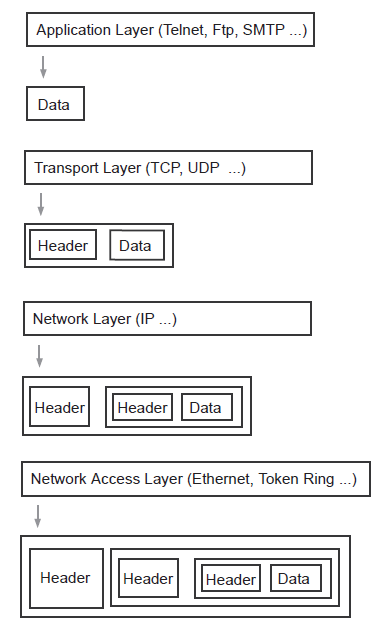
\includegraphics[width =.8\textwidth]{TCP_IP_Protocol_Stack_4_Layer_Model}
				\caption{TCP/IP Protocol.}
				\label{Fig:TCP/IP}
			\end{figure}
		
			TCP/IP uses the client/server model of communication in which a computer user (a client) requests and is provided a service (such as sending a Web page) by another computer (a server) in the network. TCP/IP communication is primarily point-to-point, meaning each communication is from one point (or host computer) in the network to another point or host computer. TCP/IP and the higher-level applications that use it are collectively said to be "stateless" because each client request is considered a new request unrelated to any previous one (unlike ordinary phone conversations that require a dedicated connection for the call duration). Being stateless frees network paths so that everyone can use them continuously. (Note that the TCP layer itself is not stateless as far as any one message is concerned. Its connection remains in place until all packets in a message have been received.)
			
			\item Protocol
			A protocol is the special set of rules that end points in a telecommunication connection use when they communicate. Protocols specify interactions between the communicating entities. 
			Protocols exist at several levels in a telecommunication connection. For example, there are protocols for the data interchange at the hardware device level and protocols for data interchange at the application program level. In the standard model known as Open Systems Interconnection (OSI), there are one or more protocols at each layer in the telecommunication exchange that both ends of the exchange must recognize and observe. Protocols are often described in an industry or international standard.
			
			The TCP/IP Internet protocols, a common example, consist of:
			Transmission Control Protocol (TCP), which uses a set of rules to exchange messages with other Internet points at the information packet level
			Internet Protocol (IP), which uses a set of rules to send and receive messages at the Internet address level
			Additional protocols that include the Hypertext Transfer Protocol (HTTP) and File Transfer Protocol (FTP), each with defined sets of rules to use with corresponding programs elsewhere on the Internet
			
			\item The Protocol Used In ZagHexa Robot
			
			Client will send "I" character in the first time of connection, Server will reply by an array of string in this format {"Sensor1\_name, ID, Sensor2\_name,ID, ..etc"}
			Ex:	{"gyroscope, 3, GPS, 4, ..etc"}
			
			Client will store this array into an text file to retrieve the ID for future requests.
			Client can do one of these requests :
			\begin{itemize}
				\item "A" character  to send all sensors data.
				\item ID number to select one sensor to get its data.
			\end{itemize}
				
			Server will reply in the first case by an array of numbers in the same order of the sensors in the index file, in the second case it will reply by a single float number that its index match the request one.
			
		\end{itemize}


\section{Sonar System}
\subsection{\textbf{Components needed:}}

\begin{enumerate}
\item  Ultrasonic sensor
\item  PIR sensor
\item  Servo motor
\item  Arduino board
\item  Jump wires
\end{enumerate}
\subsection{\textbf{Circuit scheme:}}
\begin{figure}[h]
	\centering
	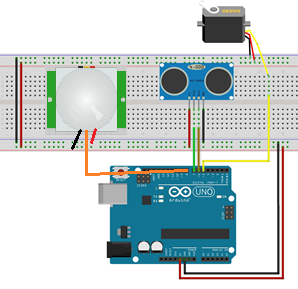
\includegraphics{figures/sonar}
\end{figure}
The Ultrasonic Sensor is connected to the pins number 4 and 5, PIR to pin 7 and the servomotor to the pin number 6 on the Arduino Board. 

Now we need to make a code and upload it to the Arduino Board that will enable the interaction between the Arduino and the Processing IDE.

\textbf{Hints about processing:}

\begin{enumerate}
\item \textbf{ }The Processing Development Environment (PDE) makes it easy to write Processing programs. Programs are written in the text editor and started by pressing the run button. 

\item  In Processing, a computer program is called a sketch. Sketches are stored in the Sketchbook, which is a folder on your computer. Sketches can draw two- and three-dimensional graphics.

\item  Processing has different programming modes to make it possible to deploy sketches on different platforms and program in different ways. The Java mode is the default. Other programming modes may be downloaded by selecting "Add Mode''.
\end{enumerate}

The Target is to make the calculation of distance, moving servo and publishing angle and PIR give the signal if it detected something to the serial port.

So as processing can handle and read their values and process them to get the output.

This is simply demonstrated in this figure:

\begin{figure}[h]
	\centering
	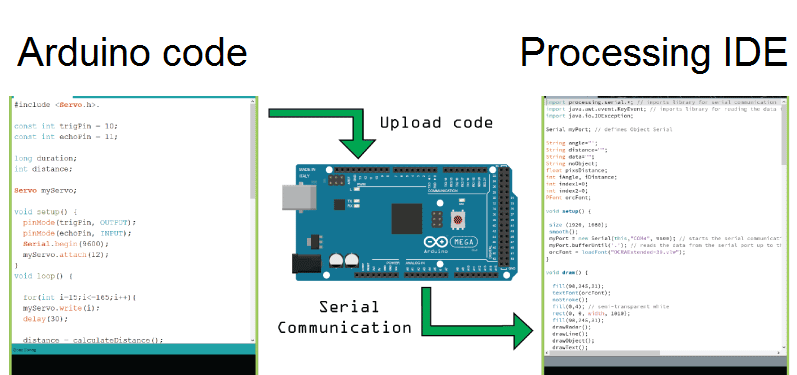
\includegraphics[width=14cm,height=7cm]{figures/sonar2}
\end{figure}
After uploading the code to Arduino and checked that the output on serial with the required pattern.

Now we will receive the values for the angle and the distance measured by the sensor from the Arduino Board into the Processing IDE using the SerialEvent() function which reads the data from the Serial Port and we will put the values of the PIR, angle and the distance into the variables myPIR, myAngle and myDistance.

These variables will be used for drawing the sonar, the lines, the detected objects{\dots}etc.

For drawing the sonar main screen, this function~was made \textbf{drawRadar()}~which consist of~\textbf{arc()}~and~\textbf{line()} functions as you see in the next figure.
They are 4 half circles and lines to demonstrate the degrees meter.
\begin{figure}[h]
	\centering
	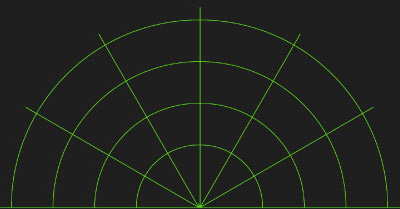
\includegraphics[width=14cm,height=7cm]{figures/sonar3}
\end{figure}
For drawing the line that is moving along the radar this function \textbf{drawLine(). }Its center of rotation is set with the \textbf{translate() }function and using the line() function in which the myAngle variable is used the line is redrawn for each degree.
\begin{figure}[h]
	\centering
	
\includegraphics[width=14cm,height=7cm]{figures/sonar4}
\end{figure}\\\\\\
 For drawing the detected objects this function \textbf{drawObject()} gets the distance from ultrasonic sensor, transforms it into pixels and in combination with the angle of the sensor draws the object on the sonar.

\begin{figure}[h]
	\centering
	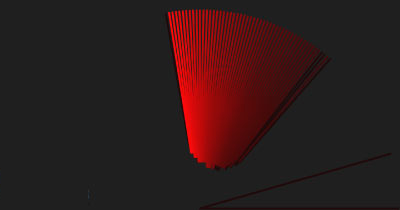
\includegraphics[width=14cm,height=7cm]{figures/sonar5}
\end{figure}

For the text on the screen the function \textbf{drawText()} draws texts on particular locations. All of these functions are called in the main \textbf{draw()} function which repeats all the time and draws the screen. 

And the final output as you can see 
\begin{figure}[h]
	\centering
	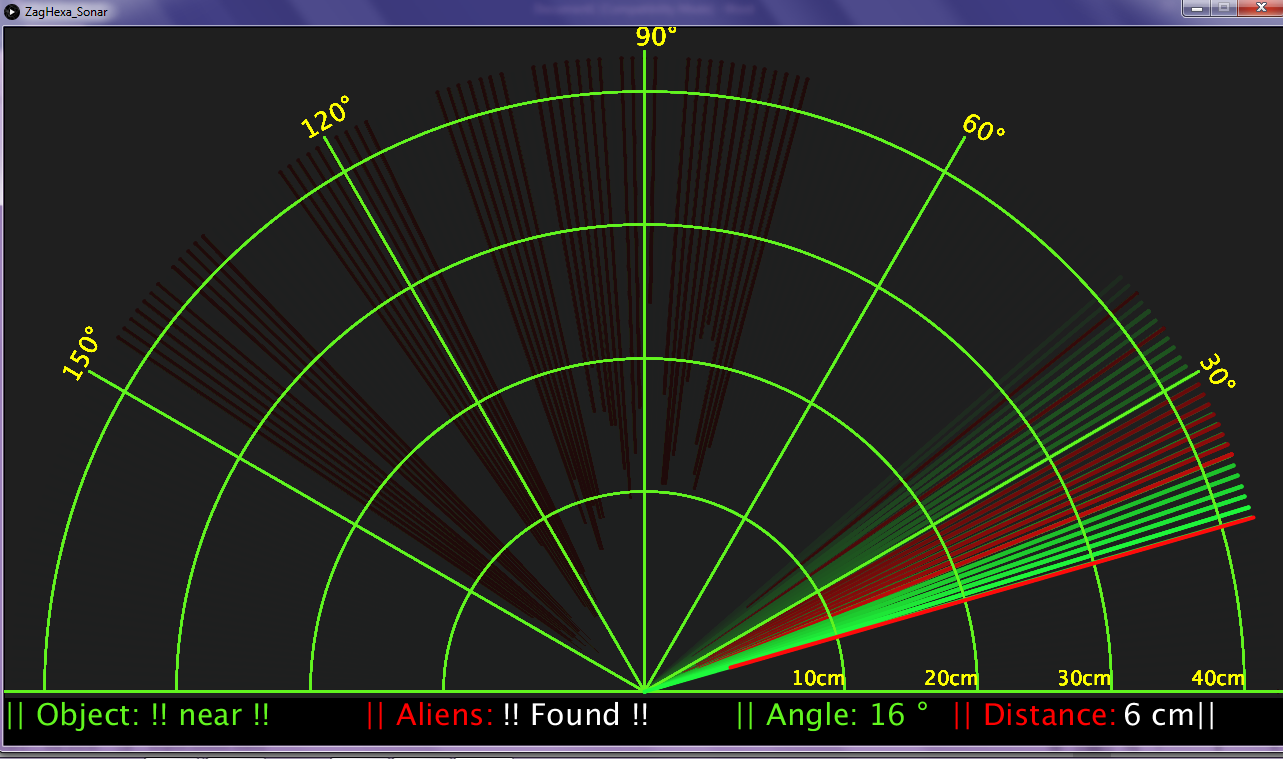
\includegraphics[width=14cm,height=8cm]{figures/sonar6}
\end{figure}

\section{GUI}

Future work